\documentclass[tikz,border=25pt]{standalone}
\usepackage{tikz}
\usepackage{amsmath}
\usepackage{amssymb}
\usepackage{helvet}
\renewcommand{\familydefault}{\sfdefault}
\usetikzlibrary{calc, positioning, arrows.meta, decorations.pathmorphing, shapes.geometric}

\definecolor{emeraldpine}{HTML}{1A4D3E}
\definecolor{harvardcrimson}{HTML}{A51C30}
\definecolor{ethdarkblue}{HTML}{1F407A}
\definecolor{ethpetrol}{HTML}{007A87}
\definecolor{ethbronze}{HTML}{B87333}
\definecolor{ink}{HTML}{1A202C}
\definecolor{cardbg}{HTML}{F8FAFC}

\begin{document}
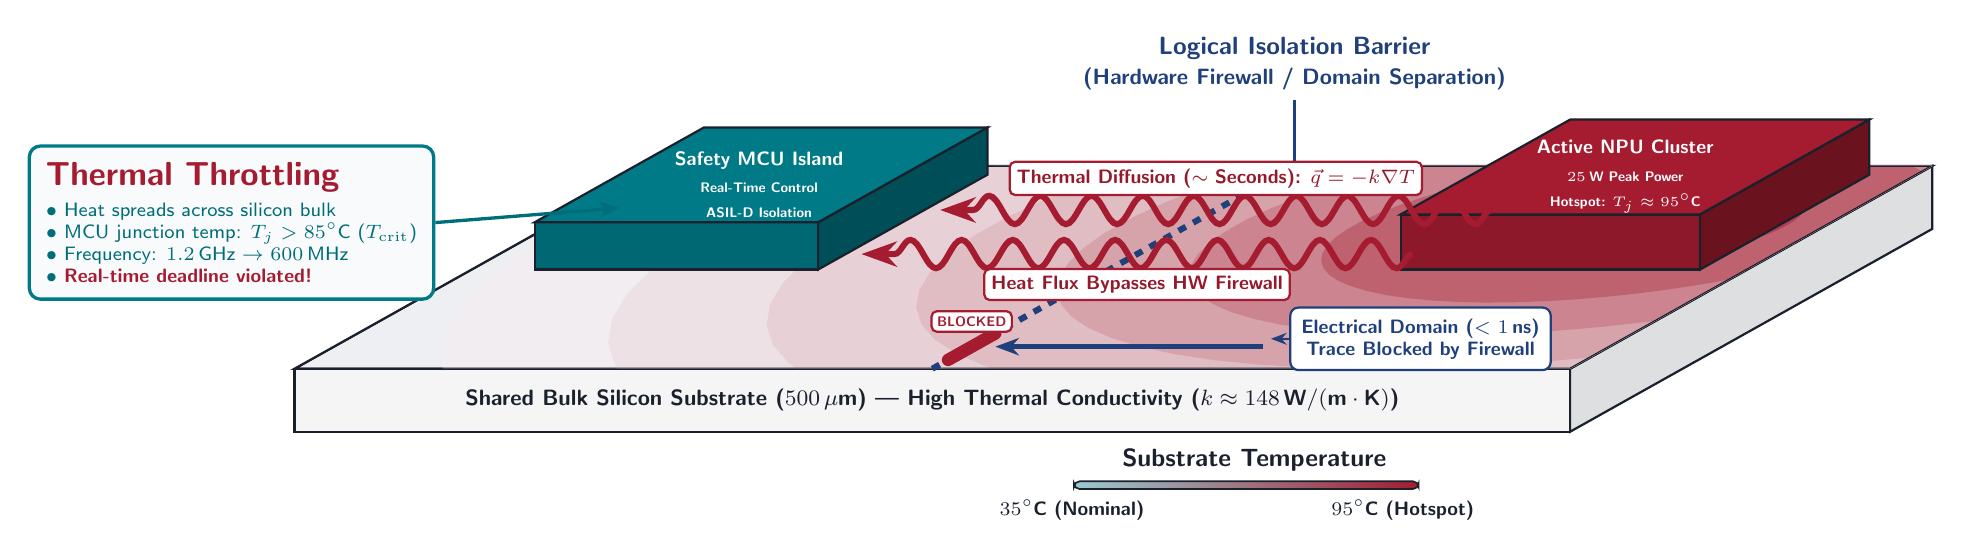
\begin{tikzpicture}[x={(1.0cm, 0.0cm)}, y={(0.50cm, 0.28cm)}, z={(0.0cm, 1.0cm)}, font=\sffamily]

  % Substrate Dimensions
  \def\SX{16.2}
  \def\SY{9.2}
  \def\SZ{0.8}

  % 1. Substrate Solid Block
  % Front face (Y = 0)
  \filldraw[fill=cardbg!80!ink!20, draw=ink, line width=0.8pt] 
    (0, 0, 0) -- (\SX, 0, 0) -- (\SX, 0, \SZ) -- (0, 0, \SZ) -- cycle;
  % Right face (X = \SX)
  \filldraw[fill=cardbg!60!ink!35, draw=ink, line width=0.8pt] 
    (\SX, 0, 0) -- (\SX, \SY, 0) -- (\SX, \SY, \SZ) -- (\SX, 0, \SZ) -- cycle;
  % Top face (Z = \SZ)
  \filldraw[fill=cardbg!95!ink, draw=ink, line width=0.8pt] 
    (0, 0, \SZ) -- (\SX, 0, \SZ) -- (\SX, \SY, \SZ) -- (0, \SY, \SZ) -- cycle;

  % Substrate front face label
  \node[font=\sffamily\footnotesize\bfseries, color=ink] at (\SX*0.5, 0, \SZ*0.5) 
    {Shared Bulk Silicon Substrate ($500\,\mu\text{m}$) --- High Thermal Conductivity ($k \approx 148\,\text{W}/(\text{m}\cdot\text{K})$)};

  % 2. Thermal Diffusion Contours on Top Face (Z = \SZ)
  \begin{scope}
    \clip (0, 0, \SZ) -- (\SX, 0, \SZ) -- (\SX, \SY, \SZ) -- (0, \SY, \SZ) -- cycle;
    % NPU center is at (13.7, 6.5)
    \foreach \r/\c in {
      13.5/6,
      11.6/12,
      9.8/20,
      8.1/30,
      6.5/42,
      5.0/56,
      3.5/72,
      2.0/88
    } {
      \fill[harvardcrimson!\c!cardbg, opacity=0.8]
        plot[domain=0:360, samples=60] ({13.7 + \r*cos(\x)}, {6.5 + \r*sin(\x)}, \SZ);
    }
    % Outline of the top face restored
    \draw[ink, line width=0.8pt] (0, 0, \SZ) -- (\SX, 0, \SZ) -- (\SX, \SY, \SZ) -- (0, \SY, \SZ) -- cycle;
  \end{scope}

  % 3. Logical Isolation Barrier (at X = 8.1)
  \draw[ethdarkblue, dashed, line width=2.2pt] (8.1, 0, \SZ) -- (8.1, \SY, \SZ);
  
  % Logical Isolation label (elevated above background blocks)
  \node[ethdarkblue, font=\sffamily\bfseries\small, align=center] (iso_label) at (8.1, \SY, 2.1) 
    {Logical Isolation Barrier\\{\footnotesize(Hardware Firewall / Domain Separation)}};
  \draw[ethdarkblue, line width=1pt] (iso_label.south) -- (8.1, \SY, \SZ);

  % 4. Active NPU Cluster (Heat Source in background right)
  % Bounds: X in [11.8, 15.6], Y in [4.5, 8.8], Z in [\SZ, \SZ + 0.7]
  \def\NPUXone{11.8}
  \def\NPUXtwo{15.6}
  \def\NPUYone{4.5}
  \def\NPUYtwo{8.8}
  \def\NPUZtop{1.5}

  % Front face
  \filldraw[fill=harvardcrimson!85!black, draw=ink, line width=0.8pt]
    (\NPUXone, \NPUYone, \SZ) -- (\NPUXtwo, \NPUYone, \SZ) -- (\NPUXtwo, \NPUYone, \NPUZtop) -- (\NPUXone, \NPUYone, \NPUZtop) -- cycle;
  % Right face
  \filldraw[fill=harvardcrimson!65!black, draw=ink, line width=0.8pt]
    (\NPUXtwo, \NPUYone, \SZ) -- (\NPUXtwo, \NPUYtwo, \SZ) -- (\NPUXtwo, \NPUYtwo, \NPUZtop) -- (\NPUXtwo, \NPUYone, \NPUZtop) -- cycle;
  % Top face
  \filldraw[fill=harvardcrimson, draw=ink, line width=0.8pt]
    (\NPUXone, \NPUYone, \NPUZtop) -- (\NPUXtwo, \NPUYone, \NPUZtop) -- (\NPUXtwo, \NPUYtwo, \NPUZtop) -- (\NPUXone, \NPUYtwo, \NPUZtop) -- cycle;

  \node[white, font=\sffamily\bfseries\scriptsize, align=center] at (13.8, 6.2, \NPUZtop) 
    {Active NPU Cluster\\[2pt]{\tiny $25\,\text{W}$ Peak Power}\\[1pt]{\tiny Hotspot: $T_j \approx 95^\circ\text{C}$}};

  % 5. Safety MCU Island (Victim in background left)
  % Bounds: X in [0.8, 4.4], Y in [4.5, 8.8], Z in [\SZ, \SZ + 0.6]
  \def\MCUXone{0.8}
  \def\MCUXtwo{4.4}
  \def\MCUYone{4.5}
  \def\MCUYtwo{8.8}
  \def\MCUZtop{1.4}

  % Front face
  \filldraw[fill=ethpetrol!85!black, draw=ink, line width=0.8pt]
    (\MCUXone, \MCUYone, \SZ) -- (\MCUXtwo, \MCUYone, \SZ) -- (\MCUXtwo, \MCUYone, \MCUZtop) -- (\MCUXone, \MCUYone, \MCUZtop) -- cycle;
  % Right face
  \filldraw[fill=ethpetrol!65!black, draw=ink, line width=0.8pt]
    (\MCUXtwo, \MCUYone, \SZ) -- (\MCUXtwo, \MCUYtwo, \SZ) -- (\MCUXtwo, \MCUYtwo, \MCUZtop) -- (\MCUXtwo, \MCUYone, \MCUZtop) -- cycle;
  % Top face
  \filldraw[fill=ethpetrol, draw=ink, line width=0.8pt]
    (\MCUXone, \MCUYone, \MCUZtop) -- (\MCUXtwo, \MCUYone, \MCUZtop) -- (\MCUXtwo, \MCUYtwo, \MCUZtop) -- (\MCUXone, \MCUYtwo, \MCUZtop) -- cycle;

  \node[white, font=\sffamily\bfseries\scriptsize, align=center] at (2.8, 6.2, \MCUZtop) 
    {Safety MCU Island\\[2pt]{\tiny Real-Time Control}\\[1pt]{\tiny ASIL-D Isolation}};

  % 6. Fast Electrical Interconnect vs Firewall (Foreground, Y = 1.0)
  % Interconnect trace on top of substrate
  \draw[-{Stealth[length=3mm, width=2.2mm]}, ethdarkblue, line width=2pt] (11.8, 1.0, \SZ) -- (8.4, 1.0, \SZ);
  % Firewall blocking bar at X = 8.1
  \draw[harvardcrimson, line width=4.5pt, line cap=round] (8.1, 0.4, \SZ) -- (8.1, 1.6, \SZ);
  
  % Blocked badge (placed directly above the firewall bar)
  \node[harvardcrimson, font=\sffamily\bfseries\tiny, fill=white, draw=harvardcrimson, line width=0.8pt, inner sep=2pt, rounded corners=2pt] 
    at (8.1, 1.0, \SZ+0.32) {BLOCKED};

  % Electrical trace callout box (in foreground, at Y = 1.0, X = 13.8)
  \node[ethdarkblue, font=\sffamily\scriptsize\bfseries, fill=white, draw=ethdarkblue, line width=0.8pt, rounded corners=3pt, inner sep=4pt, align=center] 
    (elec_box) at (13.8, 1.0, \SZ+0.1) {Electrical Domain ($< 1\,\text{ns}$)\\Trace Blocked by Firewall};
  \draw[-{Stealth[length=2mm]}, ethdarkblue, line width=0.8pt] (elec_box.west) -- (11.9, 1.0, \SZ+0.1);

  % 7. Thermal Conduction Heat Flux (Two continuous wavy arrows with dedicated positions)
  % Upper wavy arrow at Y = 7.2
  \draw[-{Stealth[length=4.5mm, width=3.2mm]}, harvardcrimson, line width=2.2pt, decorate, decoration={snake, amplitude=1.8mm, segment length=6.5mm, post length=4mm}] 
    (11.6, 7.2, \SZ) -- (4.6, 7.2, \SZ)
    node[midway, above=5pt, harvardcrimson!90!black, font=\sffamily\bfseries\scriptsize, fill=white, draw=harvardcrimson, line width=0.8pt, rounded corners=2pt, inner sep=2.5pt] 
    {Thermal Diffusion ($\sim\text{Seconds}$): $\vec{q} = -k \nabla T$};

  % Lower wavy arrow at Y = 5.2
  \draw[-{Stealth[length=4.5mm, width=3.2mm]}, harvardcrimson, line width=2.2pt, decorate, decoration={snake, amplitude=1.8mm, segment length=6.5mm, post length=4mm}] 
    (11.6, 5.2, \SZ) -- (4.6, 5.2, \SZ)
    node[midway, below=5pt, harvardcrimson!90!black, font=\sffamily\bfseries\scriptsize, fill=white, draw=harvardcrimson, line width=0.8pt, rounded corners=2pt, inner sep=2.5pt] 
    {Heat Flux Bypasses HW Firewall};

  % 8. Thermal Throttling / Consequence Card (Placed clearly to the left of substrate)
  \node[ethpetrol!90!black, font=\sffamily\scriptsize, fill=cardbg, draw=ethpetrol, line width=1.2pt, rounded corners=4pt, inner sep=6pt, align=left] 
    (throttle_card) at (-3.4, 5.2, 1.2) {
      \textbf{\color{harvardcrimson}\large Thermal Throttling}\\[3pt]
      $\bullet$ Heat spreads across silicon bulk\\
      $\bullet$ MCU junction temp: $T_j > 85^\circ\text{C}$ ($T_{\mathrm{crit}}$)\\
      $\bullet$ Frequency: $1.2\,\text{GHz} \to 600\,\text{MHz}$\\
      $\bullet$ \textbf{\color{harvardcrimson}Real-time deadline violated!}
    };
  \draw[-{Stealth[length=2.5mm, width=2mm]}, ethpetrol!90!black, line width=1.2pt] 
    (throttle_card.east) -- (\MCUXone, {(\MCUYone+\MCUYtwo)/2}, \MCUZtop*0.7);

  % 9. Temperature Scale / Legend (Bottom right, clearly below substrate front face)
  \begin{scope}[shift={(11.2, -2.6, 0)}]
    \shade[left color=ethpetrol!40, right color=harvardcrimson, rounded corners=2pt] (0, 0) rectangle (4.2, 0.35);
    \draw[ink, line width=0.6pt, rounded corners=2pt] (0, 0) rectangle (4.2, 0.35);
    \node[ink, font=\sffamily\scriptsize\bfseries, anchor=north] at (0, -0.05) {$35^\circ\text{C}$ (Nominal)};
    \node[ink, font=\sffamily\scriptsize\bfseries, anchor=north] at (4.2, -0.05) {$95^\circ\text{C}$ (Hotspot)};
    \node[ink, font=\sffamily\small\bfseries, anchor=south] at (2.1, 0.38) {Substrate Temperature};
  \end{scope}

\end{tikzpicture}
\end{document}
